\documentclass[a4paper,11pt]{article}

% Also allow to change to "Backend Library" if needed
\newcommand{\BL}{"Black Library"}

% Will be used by sec-documentation-control
\newcommand{\doctype}{Cahier des charges}
\newcommand{\docversion}{1.0}
\newcommand{\docref}{CDC\_2012\_FR\_Rathaxes}
\newcommand{\docstatus}{En attente de validation}

\usepackage[utf8]{inputenc}
\usepackage[american]{babel}
\usepackage{array,
            fancyhdr,
            graphicx,
            indentfirst}
\usepackage[pdftex,
            colorlinks=true,
            pdftitle={Cahiers des charges 2012 Rathaxes},
            pdfauthor={Équipe Rathaxes 2012}]{hyperref}

\pagestyle{fancy}
\lhead{
\includegraphics[height=1.2cm]{../images/logo_epitech}}
\chead{Rathaxes \\ \doctype}
\rhead{
\includegraphics[height=1.2cm]{../images/logo_rathaxes}}

\setlength{\headheight}{38.22325pt} % there I fixed it

\title{Cahier des charges 2012 Rathaxes}
\author{Équipe Rathaxes 2012}

\begin{document}

\begin{titlepage}
\begin{center}\leavevmode
\null
\vfill
{\LARGE Rathaxes 2012 --- Cahier des charges}%
\vskip 1cm
{\Large Rathaxes 2012 Team}%
\vskip 1cm
{\Large \today}%
\vskip 2cm

\includegraphics[height=5cm]{../images/logo_rathaxes}
\vskip 1cm
\begin{abstract}
Rathaxes traduit des descriptions de périphérique matériel et des patrons C en
pilote matériel pour Windows 7, Linux et OpenBSD.

L'électronique et la programmation sont separes dans des fichiers de
description et des patrons C.

Cette conception permet de réutiliser du code entre différents pilote matériel
ce qui réduit le temps de développement et les bogues.
\end{abstract}
\vfill
\null
\end{center}
\end{titlepage}


\section*{Contr\^ole de la documentation}

\begin{table}[h]
\begin{center}

\caption{Information sur le projet}
\begin{tabular}{|m{0.3\textwidth}|m{0.6\textwidth}|}
\hline
Groupe : & Rathaxes \\
\hline
Nom du projet : & Rathaxes \\
\hline
Type de document : & \doctype \\
\hline
Version : & \docversion \\
\hline
Référence : & \docref \\
\hline
Statut du document : & \docstatus \\
\hline
\end{tabular}

\end{center}
\end{table}

\begin{table}[h]
\begin{center}

\caption{Diffusion}
\begin{tabular}{|m{0.2\textwidth}|m{0.4\textwidth}|m{0.3\textwidth}|}
\hline
Personne & Courriel & Rôle \\
\hline
 & & \\
\hline
 & & \\
\hline
\end{tabular}

\end{center}
\end{table}

\begin{table}[h]
\begin{center}

\caption{Historique du document}
\begin{tabular}{|m{0.1\textwidth}|m{0.2\textwidth}|m{0.27\textwidth}|m{0.27\textwidth}|}
\hline
Version & Date & Nom & Description \\
\hline
0.5 & 01/07/2010 & Thomas L. & Version initiale \\
\hline
0.9 & 05/07/2010 & David, Zoltan & Dernière version française \\
\hline
1.0 & 14/07/2010 & Thomas S., Louis & Version finale \\
\hline
\end{tabular}

\end{center}
\end{table}

\clearpage


\tableofcontents
\newpage

\section{Introduction}

Ce document représente le cahier des charges pour le projet \emph{Rathaxes
2012}. Il comporte une description du travail à accomplir pour achever ce
projet. Le projet Rathaxes est un générateur de pilote matériel
multi-plateformes.

Il est réalisé par l'équipe EIP Rathaxes 2012 et s'inscrit dans la continuité
du travail effectué par l'équipe 2009.

Ce document s'adresse aux développeurs Rathaxes et à l'équipe du laboratoire
EIP. Il décrit le projet Rathaxes, ses buts, ses moyens et ses limites.

Ce projet a commencé et continue en partenariat avec le LSE (\emph{Laboratoire
Système Epita/Epitech}).

\section{Rathaxes 2009}

\subsection{Problématique}

Écrire un pilote matériel requiert des connaissances approfondies sur comment le
matériel et le système fonctionnent. Les pilotes sont lancés avec un haut niveau
de privilège et peuvent causer des désastres si quelque chose est mal fait
(arr\^et brutal de la machine)\cite{linux-tutorial}.

Chaque plateforme propose ses propres interfaces de communication et les
pilotes doivent être écrits pour chacune d'elles.

Au final, il semble évident que des logiciels sont manquants pour contrer ces
problèmes :
\begin{itemize}
\item Séparation entre les compétences matériel et logicielle ;
\item Temps de développement ;
\item Réutilisation du code.
\end{itemize}

\subsection{Vue d'ensemble du projet}

Le projet est divisé en quatre parties :
\begin{enumerate}
\item Le DSL\footnote{\emph{Domain Specific Language}} qui décrit un pilote
périphérique.
\item La \BL\ est une bibliothèque de patrons utilisée lors de la génération
du pilote.
\item Un compilateur qui traduit le DSL Rathaxes et génère un pilote.
\item Une documentation abondante sur le langage et la \BL\ pour les
utilisateurs et contributeurs de Rathaxes.
\end{enumerate}

Le DSL et le compilateur sont distribués sous licence GPLv3\cite{GPLv3} et
la \BL\ sous licence BSD\cite{BSD}.

Actuellement, Rathaxes est une preuve de concept qui peut seulement générer un
pilote RS-232.

\section{Objectif pour 2012}

A la fin de la session EIP 2012, le projet devra être utilisable par n'importe
quel programmeur de pilote avec des exemples sur du matériel actuel.

Le projet suivra plusieurs étapes qui comportent :
\begin{enumerate}
\item Des recherches sur la sémantique des bus (comme PCI, USB, i2c, \ldots) ;
\item Implémentation des bus et de leurs algorithmes dans le DSL ;
\item Ajouter de nouveaux patrons dans la \BL.
\end{enumerate}

% XXX: scene ca fait trop soutenu ici, doit on rajouter des exemples (RMLL)
Tout au long du projet, l'équipe Rathaxes sera présente sur la scène open
source.

\section{Requirements}

\subsection{The DSL}

The Rathaxes DSL must:
\begin{itemize}
\item be able to simply and robustly describes a peripheral driver;
\item be able to embed C code snippets;
\item be as natural as possible for a programmer and an electronics engineer;
\item have a robust syntax and a strong semantic.
\end{itemize}

The generated C code must be robust since the whole operating system can depend on
it.

\subsection{The Compiler}

With multi-platform, code reuse-ability and development time are at stake. The
Rathaxes driver generator must for each supported operating system:
\begin{itemize}
\item be installable on each supported operating system;
\item be able to run from the command line;
\item check for the syntax of its input against the DSL syntax;
\item check for the semantic of its input;
\item use CodeWorker\cite{CodeWorker};
\item use native tools (compiler and libraries for example);
\item generate working C code from its input and the \BL.
\end{itemize}

\subsection{The \BL}

The \BL\ must:
\begin{itemize}
\item contain code templates used by the compiler;
\item be supplemented with support for new buses;
\item be able to be upgraded with new version of the compiler.
\end{itemize}

\subsection{Asynchronous support}

Currently, Rathaxes only support synchronous communication with peripherals.
However, most peripherals use asynchronous communications (like USB) and its
support in the driver generator and the DSL is mandatory.

\subsection{New peripheral drivers}

At the end of the project new peripheral drivers should be available:
\begin{itemize}
\item USB mouse;
\item USB storage key;
\item Ethernet network card;
\item Sensors support over i2c.
\end{itemize}

\subsection{Licensing}

As a scientific project Rathaxes is distributed under two open source license:
\begin{description}
\item[GPLv3:] for the compiler in order to keep full intellectual property;
\item[BSD:] for the \BL\ in order to ease future adoption by the industry.
\end{description}

\section{Contrôle du projet}

\subsection{Statut de l'association}

Rathaxes est une association loi de 1901. Une mise à jour des statuts est
prévue pour fin 2010.

Un compte en banque géré par l'association sera créé afin de subvenir aux
besoins du projet.

Dépenses prévues :
\begin{itemize}
\item Achat de périphériques (souris, carte réseaux, \ldots) ;
\item Voyage (RMLL\footnote{Rencontres Mondiales du Logiciel
Libre(\url{http://rmll.info/}).},
Fosdem\footnote{\url{http://www.fosdem.org/}.}) ;
\item Nom de domaine (rathaxes.org).
\end{itemize}

En tant qu'association, Rathaxes peut recevoir des donations.

\subsection{Environnement de travail}

\begin{itemize}
\item Le LSE est capable de subvenir à la plupart des besoins en matériel ;
\item Trois systèmes d'exploitation seront utilisés pour les recherches et les
tests, trois machines x86 seront donc nécessaires. Cependant elles pourront
être virtualisées afin d'unifier l'environnement de test;
\item Les périphériques de test seront obtenus à partir du LSE ou achetés si
besoin;
\item Le code est hébergé sur GoogleCode à l'adresse :
\url{http://code.google.com/p/rathaxes/} ;
\item Le wiki du google code propose un point de départ pour installer et
tester Rathaxes ;
\item Le code est versionné avec
Mercurial\footnote{\url{http://mercurial.selenic.com/}.} ;
\item Le gestionnaire de bogues (tickets) est public et utilisé pour développer
le projet ;
\item Le code, les tickets ainsi que la documentation doivent être écrits en
anglais ;
\item En plus des courriels EPITECH, chaque membre du projet doit être présent
sur le canal IRC suivant: \url{irc://rathaxes@irc.freenode.org}.
\end{itemize}

\subsection{Planification}

Rathaxes 2012 est la somme de plusieurs étapes :

\begin{enumerate}
\item Étudier des pilotes existant sur chaque plateforme ;
\item Écrire des pilotes sur chaque plateforme ;
\item Définir les concepts à implémenter dans le DSL ;
\item Commencer \`a travailler avec le code de Rathaxes
\item Mettre \`a jour le DSL ;
\item Écrire des pilotes avec Rathaxes ;
\item Participer aux RMLL et Fosdem.
\end{enumerate}

\begin{center}

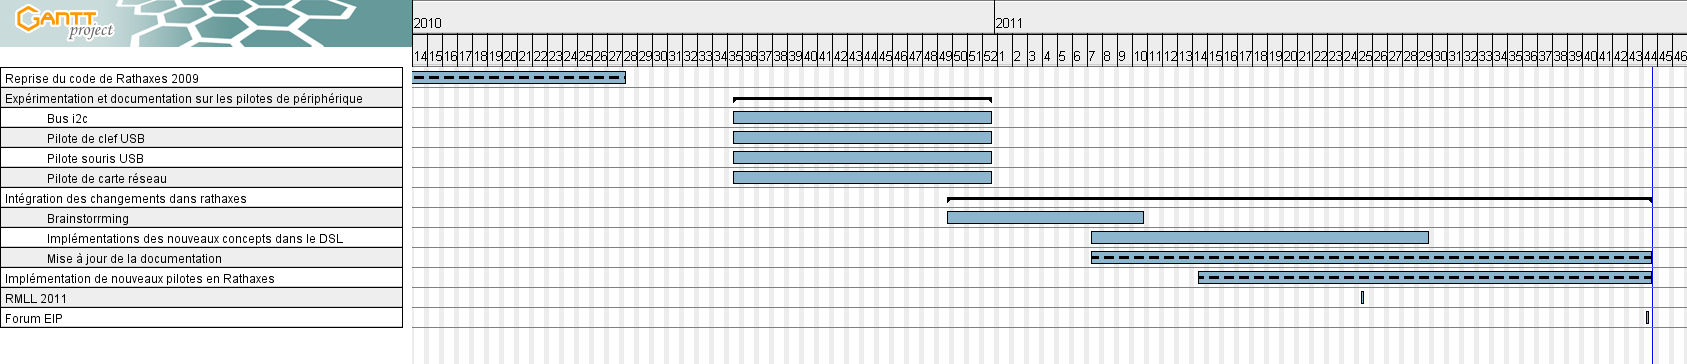
\includegraphics[angle=90,scale=0.35]{../images/gantt}

\end{center}

\begin{thebibliography}{9}

\bibitem{linux-tutorial}
The linux tutorial,
Device Driver Basic,\\
\url{http://www.linux-tutorial.info/modules.php?name=MContent&pageid=255}

\bibitem{GPLv3}
The Free Software Foundation,
\emph{GNU General Public License},\\
\url{http://www.gnu.org/licenses/gpl-3.0.html},\\
Version~3,
June~2007.

\bibitem{BSD}
University of California, Berkeley,
\emph{Simplified BSD License},\\
\url{http://www.opensource.org/licenses/bsd-license.php}.

\bibitem{CodeWorker}
A universal parsing tool \& a source code generator,\\
\url{http://codeworker.org/}.

\end{thebibliography}


\end{document}
